\documentclass[../rzero]{subfiles}
\begin{document}
\chapter{Quantum Mechanics}\label{quantumMechanicsChapter}

\begin{chapquote}{Eric Weinstein talking to Brian Keating, \textit{Youtube\cite{drbriankeatingEricWeinsteinTheoretical2020}}}
``You guys need more money. You struck the worlds worst licening deal.''
\end{chapquote}

\section{Madelung 1927}
While quantum mechanics was becoming the buzz in physics, Madelung\cite{E.Madelung1927} tried to break the field open into the direction it should have gone (and yes that is my opinion). 1927:
\begin{quotation}
	It is shown that the Schrödinger equation for one-electron problems can be transformed into the form of hydrodynamical equations.
\end{quotation}

His observation was that one can take the Schrödinger equation and pull it apart into two equations involving real phenomena, without the pesky $i \equiv \sqrt{-1}$ that causes undergrads all that trouble. 

Turns out $i$ is often concered with drag or honey, etc. So hydrodynamics drops right out of quantum mechanics, if you let it.  

We all know the outcome of that, Madelung was footnoted away, and complex algebra in quantum mechanics became so ingrained in the mind of the standard model physicist\cite{NotYourStandard} that now they are saying it's required!\cite{avellaQuantumMechanicsMust2022} No, American Physical Society $i$ is not required.\cite{mckagueSimulatingQuantumSystems2008}. If you want a simpleton explanation (i.e. by me) you can have a look at the American Physical Society paper and see if the hydrodynamic formulation is mentioned. It's not. The American Physical Society paper does have this 'get out of jail free' scentence in it, though: 

\begin{quotation}
	As Renou and his co-workers point out, these results would not be applicable to alternative formulations of quantum mechanics, such as Bohmian mechanics, which are based on different postulates. Therefore, these results could stimulate attempts to go beyond the standard formalism of quantum mechanics, which, despite great successes in predicting experimental results, is often considered inadequate from an interpretative point of view
\end{quotation} 

Ok - so maybe I'm being a little harsh on them. After all it's a great segue.   

\section{Emergent Quantum Mechanics}\label{emergentQMSection}
Everything, according to this thesis, is emergent, so then must be quantum mechanics. There is even an honest to goodness entire (ok small) research community publishing papers like \cite{tHooft2007},\cite{Grossing2012},\cite{acostaEMERGENTQUANTUMMECHANICS2012},\cite{Walleczek2019}, \cite{Durey2018}, \cite{Andersen2016} etc. 

These emergent quantum theories all say (including mine) that there is some underlying process or commonly a field from which quantum effects emerge.

\subsection{Hydrodynamic Quantum Analogs}

\begin{figure}\label{bushWalkerFigure}
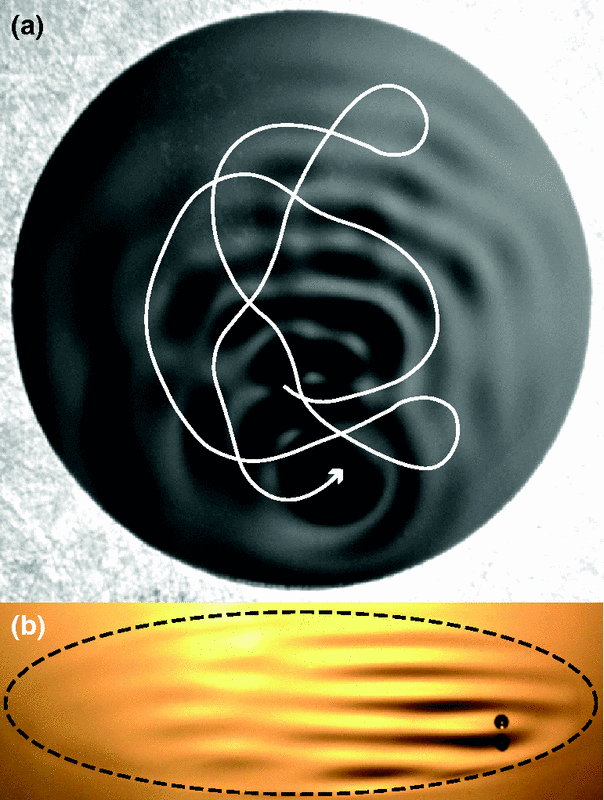
\includegraphics[width=0.45\textwidth]{chapters/images/bush-drop-path.png}
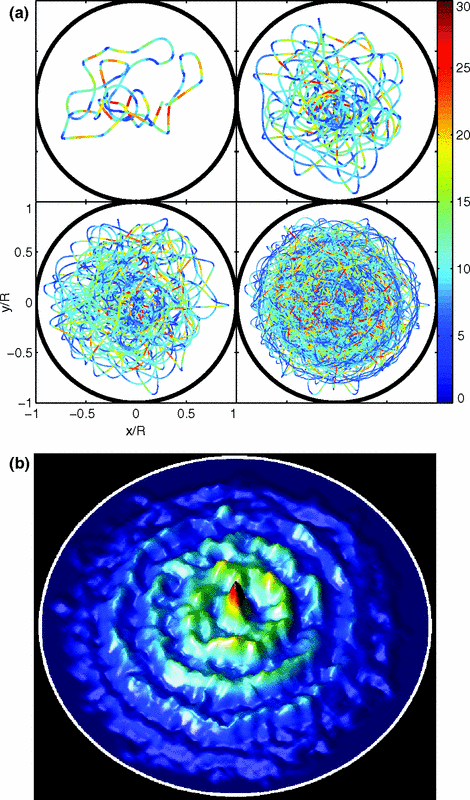
\includegraphics[width=0.45\textwidth]{chapters/images/bush-corral.png}
\caption{Walker: Bush, continuing and expanding on by earlier experiments by Couder, has shown just how a millimetre sized droplet on a vibrating bath can emulate a analagous quantum mechanical system. From\cite{harrisWavelikeStatisticsPilotwave2013} Used with permission}
\end{figure}

One of the most inspiring discoveries in theories of quantum mechanics has been the development of Hydrodynamic Quantum Analogs, which is tech speak for little (~millimeter) drops of silicon oil that 'self float' above a vibrating little bathtub (watch the videos if you don't believe me). Couder and Fort \cite{eddiInformationStoredFaraday2011} are the acknowledged pioneers of this macroscopic quantum emulation in a petri dish business. (Although I remember being at Dinty's coffee in 1986 and vibrating styro coffee cups, watching the little balls of coffee running around on top of the coffee and thinking - 'thats a great model for particle physics'.) Here are a couple of fun movies to watch - \cite{americanphysicalsocietyFaradayInstabilityFloating2014}, \cite{veritasiumThisWhatQuantum2016} 

These videos, are 'actually good'\cite{theonionYouTubeContestChallenges2008} as this comment attests:
\begin{quotation}
	Dude, I have a PhD in quantum information theory, and I've never heard of these droplets. This analogy is absolutely beautiful. 
\end{quotation}
 
This Physics Today™ article by Bush and team is great.\cite{Bush2015a}. Trust me, you will learn lots - also pretty - see figure \ref{bushWalkerFigure}.


Of course no one really thinks that quantum mechanics is powered by $10^{-19}m$ drops running around on some 2D oil bath. Although certain people have nonetheless tried to argue on that basis. Shame on them (not the reporter - the scientists, lol).\cite{wolchoverFamousExperimentDooms2018}


\subsection{The de Broglie Bohm Model}
Perhaps the most famous theory of quantum mechanics that comes to mind when one thinks about emergence, is the de Broglie - Bohm theory\cite{Bohm1952},  \cite{broglieMecaniqueOndulatoireStructure1927}, \cite{Tumulka2017}, \cite{Bohm1982}. From my point of view, de Broglie's theory is more in line with emergent QM, while Bohm showed the world that quantum mechanics can be built with particle positions and waves. In other words de Broglie was trying to build quantum mechanics from a simple underlying field, while Bohm went for a perfect replication of quantum mechanics. Both ended up at about the same place.

As J.S. Bell put it \cite{Bell1982}:
\begin{quotation}
Why is the pilot wave picture ignored in text books? Should it not be taught, not as the only way, but as an antidote to the prevailing complacency? To show that vagueness, subjectivity, and indeterminism, are not forced on us by experimental facts, but by deliberate theoretical choice?
\end{quotation}

About the only thing I have against the pilot wave theory of Bohm is that it's \textit{too good} - it has predictions identical to that of quantum mechanics - it \textit{is} quantum mechanics, after all. The wave function of Bohm is thus also just as multidimensional as all the Hilbert spaces out there, which I think is a little suspect. But still, to me, it's the closest thing we have to what nature is really like in the quantum regime. In figure \ref{bohm-trajectories-image} one can see the traces of hundreds of particles in a two slit experiment. It was an image like this which reignited interest in Bohmian mechanics in the 1980s.  

\begin{figure}\label{bohm-trajectories-image}
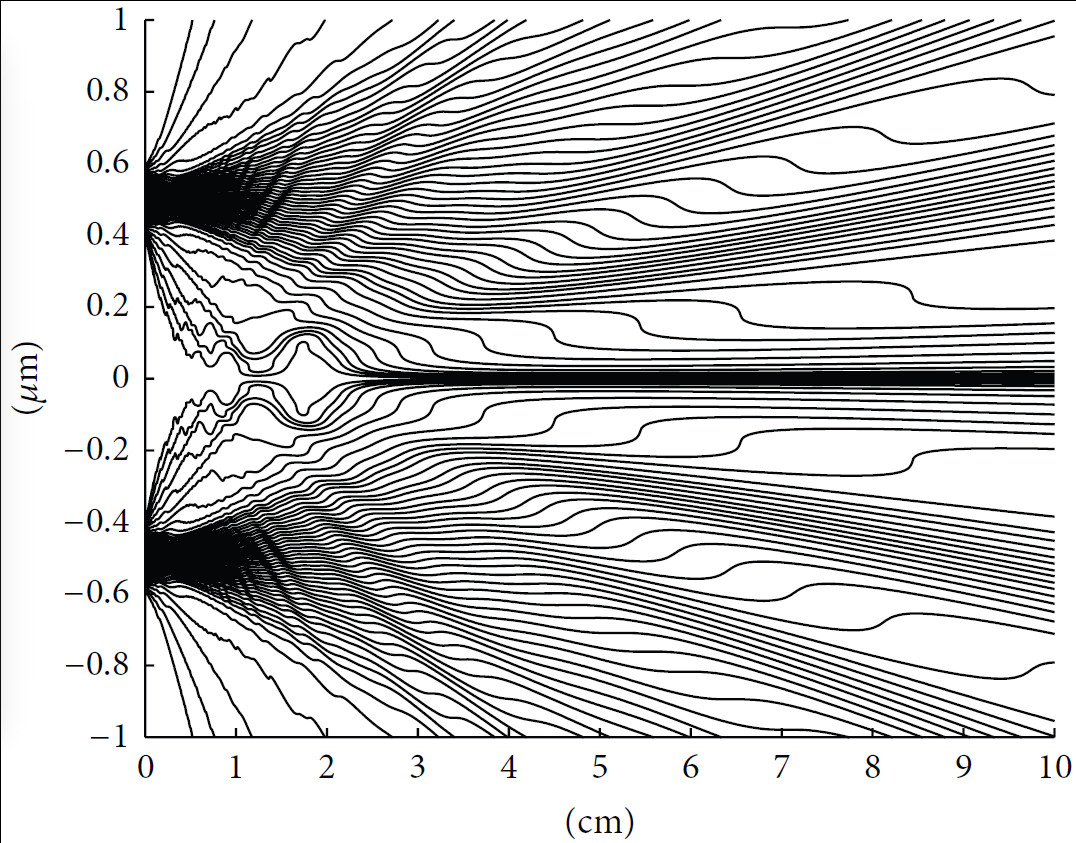
\includegraphics[width=0.65\textwidth]{chapters/images/bohmian-trajectories.png}
\caption{In de Broglie - Bohm theory, particles follow definite paths guided by the quantum potential. As J.S Bell states, there is zero indeterminacy or vagueness.   From\cite{FileBohmianTrajectories2001} Creative Commons}
\end{figure}




\subsection{Other Emergent Models of Quantum Mechanics}

So typically, and with a generous oversimplification by me, one posits some sort of field which is not quantum (remember, we are building quantum mechanics here, so it would be a little circular to  start with a quantum scalar field). Adler\cite{adlerQuantumTheoryEmergent2004} is a pioneer in the resurrection phase of this field, and Grössing is a person I admired for his attitude, leadership and organizational skills (great EmQM conferences in the mid 2010s)\cite{Grossing2012}. 

de la Peña and Cetto, have worked on a theory of emergent quantum mechanics from electromagnetism - and it's pretty nice, too.\cite{DelaPena2015}.

\begin{quotation}
	The main purpose of this book is to show that such alternative exists, and that it is tightly linked to the stochastic zero-point radiation field. This is a fluctuating field, solution of the classical Maxwell equations, yet by having a nonzero mean energy at zero temperature it is foreign to classical physics. The fundamental hypothesis of the theory here developed is that any material system is an open system permanently shaken by this field; the ensuing interaction turns out to be ultimately responsible for quantization. In other words, rather than being an intrinsic property of matter and the (photonic) radiation field, quantization emerges from a deeper stochastic process.
\end{quotation}

When authors in emergent quantum mechanics say their theory is non classical, they generally mean that the mechanism(s) required are not 'normal' classical mechanics - there are fields with no back reaction, the stochastic electromagnetic field of de la Peña and Cetto, etc.

Me, being bat crap crazy, have worked on a theory of emergent quantum mechanics from General Relativity - and it's pretty weird, too.\cite{Andersen2016}. But first let's look at some facts about quantum mechanics.

\section{An Underlying Field}
If quantum mechanics is emergent, there are two main tasks, determining the nature of the underlying field (Electromagnetism, Scalar, General Relativity) and on top of that field, the rules and regulations that allow that field to create experimental results that match what the standard quantum theory predicts. 

Of course the two steps are interrelated. What I'm getting at here is that if one were to find my theory of the underlying material field as Einstein's Ether\cite{Einstein1920} (General Relativity), tenable, then hopefully you won't tie that to my interpretation of what makes it all go. 

\section{Experimental Relality}
What do we know about quantum mechanics?

\begin{enumerate}
	\item{Quantum mechanics works faster than light.}\label{qmFasterThanC}
	\item{The normal stuff that they teach in uni}
\end{enumerate}

One might think I put item (\ref{qmFasterThanC}) in there just to get proper standard model physicists upset. But I really believe it -  from an experimental viewpoint, quantum mechanics is 'non local'. The Nobel Committee agrees\cite{AllNobelPrizes} (well they did in 2022). Here is what Maudlin has to say about it\cite{Maudlind}:

\begin{quotation}
	I retrace the history and logical structure of these arguments in order to clarify the proper conclusion, namely that any world that displays violations of Bell's inequality for experiments done far from one another must be non--local. Since the world we happen to live in displays such violations, actual physics is non--local.
\end{quotation}

Since Tim Maudlin is a philosoher, physicists can and do ignore him, or try and bury him\cite{Werner2014}, but he does fight back\cite{WMaudlin2014}. 

For me, non-locality is an imprecise description of what is going on. In the sense discussed in this book 'non local' means 'faster than light' - not acausal. Almost all physicists hold that these are equivalent ideas, because any faster than light effect can be looked at in a frame that violates causality, but as Sabine Hossenfelder\cite{sabinehossenfelderThinkFasterLight2023}, 'Dialect'(who is that?)\cite{dialectWhatTimeDilation2023} and this fine gentleman, Lukas Rafaj (reluctantly)\cite{physics-problemsandsolutionsOneWaySpeed2023} point out, it's not cut and dry. There is no proof that Einstein's philosophical 'the way it is' approach to special relativity is any better than the Lorentz physical contraction theory viewpoint. 

\textbf{There may be a grand rest frame.} Special Relativity does not rule it out. It 'merely' says that we can't use light beams, rocket ships, rulers or the Large Hadron Collider to find it. (Just don't look out a window at night, you might see a rest frame!).

Look at Consoli \cite{consoliQuantumNonLocalityCMB2022a}

\begin{quotation}
	In this way, by comparing with experiments [19, 20, 21, 22, 23] one finds the lower bounds $v_{QI} > 10^4 \hyphen 10^6c$ if the preferred $\Sigma$ frame is identified with the reference system where the Cosmic Microwave Background (CMB) is seen isotropic, namely that particular system where the observed CMB Kinematic Dipole [18] vanishes exactly. 
\end{quotation}

Any theory of emergent quantum mechanics has to reproduce something like the Schrödinger equation, etc, so that all the atoms and NP gates work as they actually do. 


Us \href{https://youtu.be/p5nWKkyzh_Y?si=eSFOG0lw4fJo7tO2&t=1153}{very simple minded} folk\cite{instituteforadvancedstudySpacetimeQuantumMechanics2021} like to think of the effects of quantum mechanics in the real world most often as just de Broglie wavelength effects. So while the theory people live a more Hilbert like lifestyle, us(? am i still one?) experimenters are still dealing with waves and particles, like Issac Newton and Thomas Young.\footnote{Of course atomic physicists use the complete rules of quantum mechanics to predict the energy levels of atoms. Kudos to them to dream that they aren't chemists.} 

So I'm going to concentrate on that bit of quantum mechanics, the source of these de Broglie waves. Sort of a 1920 level of description.

\section{Quantum Mechanics from General Relativity}
Finally, I will spill the beans on what I think is happening with quantum mechanics. 

\subsection{Some sort of Emergent Quantum Mechanics holds}
I'll start by reiterating that I think that one of the extant models of emergent quantum mechanics as outlined in section \ref{emergentQMSection} above is approximately right, and quantum mechanics is riding on top of some sort of field. I'm here to sell you on General Relativity being that field. 

\subsection{General Relativity has an ability to send signals faster than light.}
What? 

Did you not read chapter \ref{monopoleGravitationalWavesChapter}? I tried to show that General Relativity, if one counts energy in a reasonable manner, might allow for a faster than light pressure wave which has a speed of $\approx \sqrt{r/m}$ (relative to the master 'Cosmic Microwave Background' frame. This wave typically has a speed of $10^4 c$, in the earth, solar system and galaxy. This pressure wave is distinct from all the light speed stuff we know, which includes:

\begin{itemize}
  \item Light (duh).
  \item Gravitational waves.
  \item Matter.
  \item Other stuff I have likely forgot about.
\end{itemize}

Matter is on the list at least experimentally, as it follows the Lorentz transformations. Basically this means that all the stuff we know and love is made of transverse waves. Well except for (according to me), the quantum mechanics stuff that seems to be in charge when it comes to many of the rules of the game. 

\subsection{The de Broglie - Compton effect}
Particles vibrate at Compton frequencies. This is an experimental fact. Dirac called it Zitterwebung, (and used a number a factor of two away from the Compton frequency, which I won't worry about). For an electron it's $\num{1.236e20} Hz$. 

As de Broglie illustrated, one can get the de Broglie wavelength..

BLAH BLAH



\subsection{Particles absorb and emit these monopole P - waves}
So these faster than light pressure waves can experience boundaries and other phenomena. The waves set up a Faraday wave pattern - as in de Broglie, Couder, Bush, etc. This exchange leads to the 'quantum potential'. 




\subsection{The de Broglie - Compton wave}
\begin{itemize}
  \item ---frequency - compton see \ref{electronModelChapter}
  \item ---de Broglie effect - well known.
 \end{itemize}


\section{Dark matter is quantum mechanics}
	All these P-waves running around - we might be able to see them. Consider a model where each particle of matter (aka nucleus, neutron, proton, etc) , 

\section{Weak force?}
	Look at a weak force model of stochastic quantum wave effects - seems doubtful... 
\end{document}
